% \documentclass{article}
\documentclass[professionalfont]{beamer}

%%%%%%%%%%%%%%%%%%%%%%%%%%%%%%%
%%% packages
\usepackage[utf8]{inputenc}
\usepackage[brazilian]{babel}
\usepackage{amssymb} %Mathematics
\usepackage{amsfonts}%Mathematics
\usepackage{amsmath,amscd}%Mathematics
\usepackage{amsthm}%Mathematics
\usepackage{mathrsfs}%Mathematics font
\usepackage{newtxtext,newtxmath}
\usepackage{xfrac}
\usepackage{cite}
\usepackage{ragged2e}
\usepackage{geometry}
\usepackage{calc}
\usepackage{graphicx}
\usepackage{tikz}
\usepackage[absolute,overlay]{textpos} % para usar textblock
\usepackage{tcolorbox}
\usepackage[absolute,overlay]{textpos}
% \usepackage[font=small,compatibility=false]{caption}
\usepackage[font=footnotesize]{subcaption}
% \usepackage{subfig}
%%%%%%%%%%%%%%%%%%%%%%%%%%%%%%%

%%%%%%%%%%%%%%%%%%%%%%%%%%%%%%
%%%% definitions
\everymath{\displaystyle}
\usetheme{Warsaw}
%%%%%%%%%%%%%%%%%%%%%%%%%%%%%%

%%%%%%%%%%%%%%%%%%
\setbeamertemplate{caption}[numbered]
%%%%%%%%%%%%%%%%%%

%%%%%%%%%%%%%%%%%%%%%
% -- citacoes --
% \usepackage[brazilian,hyperpageref]{backref}	 % Paginas com as citações na bibl
\usepackage[alf,abnt-repeated-title-omit=yes,abnt-emphasize=bf,abnt-etal-list=0]{abntex2cite}
% \usepackage[alf,abnt-repeated-title-omit=yes,abnt-etal-list=0]{abntex2cite}
\citebrackets()
% -- citacoes --
%%%%%%%%%%%%%%%%%%%%%%

\newcommand{\dia}{\today}
\newcommand{\autor}{João Paulo Rodrigues de Andrade}
\newcommand{\orientador}{Darlan Karlo Elisiário de Carvalho}
\newcommand{\titulo}{Aplicação do método Multinível Algébrico Dinâmico Não Uniforme (NU-ADM) no escoamento composicional em reservatórios de petróleo.}
\newcommand{\instituicao}{Universidade Federal de Pernambuco}


%%%%%%%%%%%%%%%%%%%%%%%%%%%%%%%%%%%%%
%% novos comandos
\let\divsymb=\div % rename builtin command \div to \divsymb
\newcommand{\gv}[1]{\ensuremath{\mbox{\boldmath$ #1 $}}}
\renewcommand{\div}[1]{\gv{\vec{\nabla}} \cdot #1} % for divergence
\newcommand{\pd}[2]{\frac{\partial #1}{\partial #2}}
\newcommand{\grad}[1]{\gv{\nabla} #1} % for gradient
%%%%%%%%%%%%%%%%%%%%%%%%%%%%%%%%%%%%%


\def \porosidade{\phi}
\def \perm{K}
\def \poroVolume{V_{p}}
\def \totalVolume{V_{b}}
% \def \permTensor{\undertilde{K}}
\def \permTensor{\underline{\underline{K}}}
\def \Volume{V}
\def \velocity{\vec{v}}
\def \permRel{kr}
\def \phase{j}
\def \pressure{P}
\def \density{\rho}
\def \viscosity{\mu}
\def \milidarcy{md}
\def \gravity{g}
\def \permEff{k_{ef}}
\def \permAbs{K_{abs}}
\def \sourceTerm{Q}
\def \normalVec{\vec{n}}
\def \volumeSurface{\Gamma_{V}}
\def \faceVolume{L}
\def \normalVersor{\hat{n}} %remover
\def \Area{A}
\def \component{k}
\def \molNumber{n}
\def \molNumberComponent{\molNumber_{\component}} %remover
\def \globalMolarFraction{z}
\def \timme{t}
\def \bulkVolume{V_{b}}
\def \numberOfPhases{N_{\phase}}
\def \numberOfComponents{N_{c}}
\def \molarPartialFrac{x}
\def \altura{D}
\def \molarDensity{\xi}
\def \molarDensityPhase{\xi_{\phase}} %remover
\def \molarDensityComponent{\molarDensity_{\component}}  %remover
\def \mSourceTerm{q}
\def \totalFluidVolume{V_{t}}
\def \porosidadeIni{\porosidade^{0}}
\def \rockCompress{c_{f}}
\def \pressureIni{\pressure_{f}}
\def \aComponent{a_{\component}} %remover
\def \aPhase{a_{\phase}} % remover
\def \alphaComponent{\alpha_{\component}} %remover
\def \bComponent{b_{\component}} %remover
\def \bPhase{b_{\phase}} %remover
\def \componentt{\component_{1}} %%remover
\def \componenttt{\component_{2}} %%remover
\def \molarVolume{v}
\def \molarphaseVolume{\molarVolume_{\phase}} %remover
\def \molarVolumeComponent{\molarVolume_{\component}}  %remover
\def \rConstant{R}
\def \temperature{T}
\def \Joule{J}
\def \mol{mol}
\def \m3{m^{3}}
\def \binaryInter{\kappa}
\def \omegaA{\Omega_{a}} %remover
\def \omegaB{\Omega_{b}} %remover
\def \Critical{c}
\def \criticalT{\temperature_{\Critical}}
\def \criticalTComponent{\temperature_{\Critical \component}} %% remover
\def \criticalP{\pressure_{\Critical}}
\def \criticalPComponent{\pressure_{\Critical \component}} %remover
\def \criticalV{\Volume_{\Critical}}
\def \crititicalVComponent{\Volume_{\Critical \component}} %remover
\def \criticalMolarDensity{\molarDensity_{\Critical}}
\def \criticalMolarDensityPhase{\molarDensity_{\Critical \phase}} %remover
\def \malphaComp{\gamma_{\component}} %remover
\def \acentricFator{\omega}
\def \acentricFatorComponent{\acentricFator_{\component}}
\def \Zfactor{Z}
\def \ZfactorPhase{\Zfactor_{\phase}} % remover
\def \BPhase{B_{\phase}} %remover
\def \APhase{A_{\phase}} % remover
\def \fugacity{f_{\component \phase}}
\def \coefFugacity{\varphi}
\def \Saturation{S}
\def \oilPhase{o} % remover
\def \waterPhase{w} %remover
\def \gasPhase{g} %remover
\def \MolecularWeight{W}
\def \MolecularWeightComponent{\MolecularWeight_{\component}} % remover
\def \MolecularWeightPhase{\MolecularWeight_{\phase}} %remover
\def \viscosityComponent{\viscosity_{\component}} %remover
\def \viscosityLowPressure{\viscosity^{*}}
\def \viscosityLowPressureComponent{\viscosityLowPressure_{\component}} %remover
\def \Reduced{r} %remover
\def \reducedTemperature{\temperature_{\Reduced}}
\def \reducedTemperatureComponent{\temperature_{\Reduced \component}}%remover
\def \reducedPressure{\pressure_{\Reduced}}
\def \reducedMolarDensity{\molarDensity_{\Reduced}}
\def \zetaParam{\zeta}
\def \zetaParamComponent{\zetaParam_{\component}}
\def \atmPressure{atm}
\def \kelvinTemperature{K}
\def \reducedMolarDensity{\molarDensity_{\Reduced}}
\def \reducedMolarDensityPhase{\molarDensity_{\Reduced \phase}}
\def \etaParam{\eta}
\def \sumInComponents{\displaystyle \sum_{\component}^{\numberOfComponents}} %remover
\def \MolarMass{M}
\def \MolarMassComponet{\MolarMass_{\component}} %remover
\def \mobility{\lambda}
\def \mobilityPhase{\mobility_{\phase}} % remover
\def \totalMobility{\mobility_{T}}

\def \coarseRatio{Cr}
\def \volf {\Omega_{i}}
\def \volfBoundary{\partial \volf}
\def \volcoarse {\Omega_{I}}
\def \volDual{\Omega_{I}^{d}}
\def \boundaryVolDual{\partial \volDual}
\def \prolOperator{\underline{\underline{OP}}}
\def \level{l}
\def \prolOperatorIi{\prolOperator^{\level}_{\level-1}}
\def \restOperator{\underline{\underline{OR}}}
\def \restOperatorIi{\restOperator^{\level-1}_{\level}}
\def \basisFunction{\phi}
\def \basisFunctionIi{\basisFunction^{I}_{i}}
\def \correctionFunc{\phi^{*}}
\def \kroneckerDelta{\delta}
\def \correctionFunci{\correctionFunc_{i}}
\def \fine{f}
\def \vectorPressure{\mathbf{\pressure}^{\fine}}
\def \vectorFinePressureWire{\bold{P}^{fw}}

\def \msPressure{\pressure'}
\def \vectorMsPressure{\bold{\pressure}'}

\def \numberFineVols{N^{f}}
\def \numberCoarseVols{N^{c}}
\def \coarsePressure{\pressure_{I}^{c}}
\def \vectorCoarsePressure{\bold{\pressure}^{c}}
\def \permutationMatrix{\underline{\underline{G}}}
\def \transmissibility{T}
\def \fineTransmissibility{\underline{\underline{\transmissibility}}^{f}}
\def \vectorfineSource{\mathbf{q}^{f}}
\def \dualInternal{i}
\def \dualFace{f}
\def \dualEdge{e}
\def \dualVertex{v}
\def \finewirebasketMatrix{\underline{\underline{M}}}
\def \MIntInt{M_{\dualInternal \dualInternal}}
\def \MIntFac{M_{\dualInternal \dualFace}}
\def \MFacInt{M_{\dualFace \dualInternal}}
\def \MFacFac{M_{\dualFace \dualFace}}
\def \MFacEdg{M_{\dualFace \dualEdge}}
\def \MEdgFac{M_{\dualEdge \dualFace}}
\def \MEdgEdg{M_{\dualEdge \dualEdge}}
\def \MEdgVer{M_{\dualEdge \dualVertex}}
\def \MVertEdg{M_{\dualVertex \dualEdge}}
\def \MVertVert{M_{\dualVertex \dualVertex}}
\def \fineWirebasketSource{b}
\def \vectorFineWirebasketSource{\bold{b}}
\def \vectorFineWirebasketSourceMod{\bold{b}'}
\def \finewirebasketMatrixMod{\underline{\underline{{\tilde{M}}}}}
\def \MFacFacMod{\tilde{M}_{\dualFace \dualFace}}
\def \MEdgEdgMod{\tilde{M}_{\dualEdge \dualEdge}}
\def \coarseTransmissibility{\underline{\underline{\transmissibility}}^{c}}
\def \correctionFunctionMatrix{\underline{\underline{C}}}
\def \coarseSourceTerm{\bold{R}^{c}}
\def \identityMatrixVert{I_{\dualVertex \dualVertex}}
\def \spaceum{\hspace{0.1cm}}
\def \refFigura{Figura}
\def \vectorIntermPressure{\bold{P}''}
\def \IntermPressure{P''}
\def \prolOperatorAdm{\hat{\prolOperator}}
\def \restOperatorAdm{\hat{\restOperator}}
\def \vectorPressureAdm{\bold{\pressure}^{ADM}}

\def \permeability{K}
\def \molarPhaseFraction{\Upsilon}


\title[NU-ADM]{Aplicação do método Multinível Algébrico Dinâmico Não Uniforme (NU-ADM) no escoamento composicional em reservatórios de petróleo}
\author[João Paulo Rodrigues de Andrade]{João Paulo Rodrigues de Andrade}
\institute[UFPE]{Universidade Federal de Pernambuco}
% \titlegraphic{
\includegraphics[scale=0.2]{./imgs/ufpe.png} \hspace{0.5cm} 
\includegraphics[scale=0.2]{./imgs/ufpe.png}}

\date{}

\newcommand\Wider[2][3em]{%
\makebox[\linewidth][c]{%
  \begin{minipage}{\dimexpr\textwidth+#1\relax}
  \raggedright#2
  \end{minipage}%
  }%
}

\setbeamersize{text margin left=0.5cm,text margin right=0.5cm}
\newlength\MyColSep
\setlength\MyColSep{1cm}
\newlength\MyColWd
\setlength\MyColWd{.5\textwidth}


\begin{document}

% {
% \setbeamertemplate{background}{%
%   \raisebox{-1cm}{%
%     \parbox[c]{3cm}{\centering%
%       
\includegraphics[width=2cm]{./imgs/ufpe.png}%
%     }%
%     \parbox[c]{\dimexpr\paperwidth-3cm\relax}{\centering%
%       {\Large The Name of the University}%
%     }%
%   }%
% }

\begin{frame}
    % \titlepage
    \begin{minipage}{\textwidth}
    
    \begin{textblock*}{5cm}(0.5cm,2.8cm) % {block width} (coords)
        
\includegraphics[scale=0.2]{./imgs/ufpe.png}
    \end{textblock*}
    
    \begin{textblock*}{8cm}(2.3cm,3.5cm) % {block width} (coords)
        \Large \instituicao
    \end{textblock*}
    
    \begin{textblock*}{5cm}(10.5cm,2.9cm) % {block width} (coords)
        
\includegraphics[scale=0.25]{./imgs/padmec.jpeg}
    \end{textblock*}
    \end{minipage}
    
    \vspace{1.8cm}
    
    \begin{minipage}{\textwidth}
        \begin{tcolorbox}[halign=center,
    valign=center,colupper=black,boxsep=1pt,width=\textwidth,colback={white},colbacktitle=yellow]    
            \Large \titulo
        \end{tcolorbox}
    \end{minipage}
    
    \vspace{0.3cm}
    
    \begin{minipage}{\textwidth}
        \autor
        
        Orientador: \orientador
    \end{minipage}
    
    \vfill
        
    Recife, \dia
    
    % João Paulo Rodrigues de Andrade
    
    % Orientador: Darlan Karlo Elisiário de Carvalho
    
    % Recife, \today
    
\end{frame}

\begin{frame}{Índice}
\begin{columns}[t]
        \begin{column}{.4\textwidth}
            \tableofcontents[sections={1-3}]
        \end{column}
        \begin{column}{.4\textwidth}
            \tableofcontents[sections={4-6}]
        \end{column}
    \end{columns}
\end{frame}

\section{Introdução}



\begin{frame}
\frametitle{Introdução}
\index{Introdução}
\begin{itemize}
    \item Importância da simulação computacional
    \item Importância da utilização de modelos composicionais
    \item Problema do tempo de simulação
    \item Métodos de Transferência de escala: \textit{Upscaling}, Multiescala, ADM
    \item Método NU-ADM
\end{itemize}
\end{frame}

\section{Objetivos}

\subsection{Geral}
\begin{frame}{Objetivos}

    \begin{block}{Geral}
        \begin{itemize}
            \item Desenvolver uma bliblioteca em Python que realize a transferência de escala, aplicando o método ADM não uniforme (NU-ADM) em modelos que lidam com escoamento composicional.
        \end{itemize}
    \end{block}
    
\end{frame}

\subsection{Específicos}
\begin{frame}{Objetivos}
    
    \begin{block}{Específicos}
        \begin{itemize}
            \item Desenvolver um interpretador os dados do reservatório
            \item Estudar o modelo de escoamento composicional
            \item Estudar o método Multiescala
            \item Estudar o método ADM e NU-ADM
            \item Aplicar o método NU-ADM no modelo composicional IMPEC
            \item Comparar a solução da malha fina com a obtida por meio do método NU-ADM
        \end{itemize}
    \end{block}
    
\end{frame}

\section{Fundamentação Teórica}

\subsection{Lei de Darcy}
\begin{frame}{Lei de Darcy}

\begin{textblock*}{.5\paperwidth}(0.2cm,2.5cm)
    \centering
    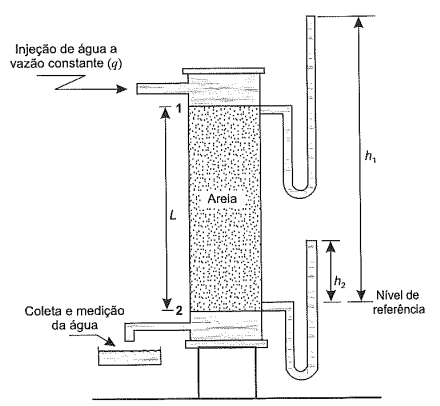
\includegraphics[scale=0.4]{./imgs/im1.png}
    \footnotesize Retirado de \cite{Rosa2006}.
\end{textblock*}

\begin{textblock*}{.48\paperwidth}(6.4cm,3cm)
    Darcy estabeleceu que, para qualquer vazão, a velocidade do fluxo é diretamente proporcional à diferença nas alturas manométricas \cite{044441830X}.
    \begin{equation}
        v = \perm \dfrac{h_{1} - h_{2}}{L}
    \end{equation}
    
    
\end{textblock*}

\end{frame}

\begin{frame}{Lei de Darcy}
    Generalizando:
    \begin{equation}
        \velocity = -\permTensor \dfrac{1}{\mu} (\grad{p} - \grad{D})
    \end{equation}
    
    \vspace{0.3cm}
    
    \begin{description}[]
        \item $\permTensor$ : tensor permeabilidade da rocha;
        \item $\velocity$: velocidade do fluido;
        \item $p$: pressão do fluido;
        \item $\mu$: viscosidade do fluido;
        \item $D$: altura do fluido
    \end{description}
    
    \begin{textblock*}{.5\paperwidth}(6cm,5cm)
        \begin{align*}
            \permTensor = 
            \begin{bmatrix}
            	K_{xx} & K_{xy} & K_{xz} \\
            	K_{yx} & K_{yy} & K_{yz} \\
            	K_{zx} & K_{zy} & K_{zz}
	        \end{bmatrix}
        \end{align*}
    \end{textblock*}
    
\end{frame}

\subsection{Método dos volumes finitos}
\begin{frame}{Método dos volumes finitos}
\begin{figure}[!ht]
\centering
    \caption{Exemplos de malhas computacionais}
    \begin{subfigure}[t]{.45\textwidth}
        \centering
        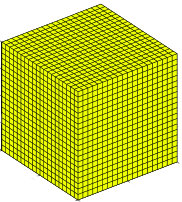
\includegraphics[scale=0.25]{./imgs/im3.png}
        \caption{3D estruturada}
        \label{fig:volumes_finitos1.a}
    \end{subfigure}
    \begin{subfigure}[t]{.45\textwidth}
        \centering
        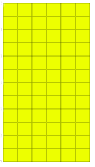
\includegraphics[scale=0.25]{./imgs/im4.png}
        \caption{2D estruturada}
        \label{fig:volumes_finitos1.b}
    \end{subfigure}
    \\
    \begin{subfigure}{.45\textwidth}
        \centering
        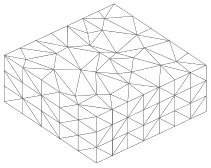
\includegraphics[scale=0.27]{./imgs/im6.png}
        \caption{3D não estruturada}
        \label{fig:volumes_finitos1.c}
    \end{subfigure}
    \begin{subfigure}{.45\textwidth}
        \centering
        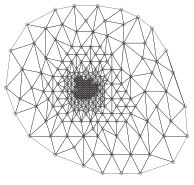
\includegraphics[scale=0.27]{./imgs/im5.png}
        \caption{2D não estruturada}
        \label{fig:volumes_finitos1.d}
    \end{subfigure}
\end{figure}

\end{frame}

\begin{frame}{Método dos volumes finitos}

\begin{columns}
\begin{column}{0.6\textwidth}
Equação do balanço de massa na forma integral:
  \begin{equation}
	\label{eq:volumes_finitos.1}
	\int_{V} \pd{\rho}{t} dV = \int_{V} - \div{(\rho \velocity)} dV + \int_{V} Q dV
\end{equation}

Aplicando o teorema de Gauss na segunda integral de \eqref{eq:volumes_finitos.1} \cite{Souza2015}:

 \begin{equation}
	 \label{eq:volumes_finitos.2}
	 \int_{V} - \div{(\rho \velocity)} dV = \int_{\volumeSurface} - \rho \velocity \cdot \normalVec \text{ } d \volumeSurface
 \end{equation}

\end{column}
\begin{column}{0.4\textwidth}  %%<--- here
    \begin{equation}
        \fineTransmissibility \vectorPressure = \vectorfineSource
    \end{equation}

    \begin{description}[]
        \small
        \item $\volumeSurface$: contorno do volume $V$;
        \item $\rho$: densidade do fluido;
        \item $Q$: termo fonte ou sumidouro;
        \item $t$: tempo;
        \item $\fineTransmissibility$: matriz transmissibilidade;
        \item $\vectorPressure$: vetor de pressão;
        \item $\vectorfineSource$: vetor do termo fonte;
        \item $^{f}$: Malha fina
    \end{description}
    
\end{column}
\end{columns}



    
\end{frame}



\subsection{Modelo Composicional}
\begin{frame}{Equações de estado}

% \begin{columns}
%     \begin{column}{0.6\textwidth}


%     \end{column}
%     \begin{column}{0.4\textwidth}  %%<--- here
%     \end{column}
% \end{columns}
    
    Nesse trabalho foi utilizada a equação de Peng-Robinson dada por \cite{Chen2007}:
    \begin{equation}
        \label{eq:eos.1}
        \pressure_{\phase} = \dfrac{\rConstant \temperature}{\molarphaseVolume - \bPhase} - \dfrac{\aPhase}{\molarphaseVolume(\molarphaseVolume + \bPhase) + \bPhase(\molarphaseVolume - \bPhase)}
    \end{equation}
    \begin{columns}
        \begin{column}{0.6\textwidth}
            \begin{description}[]
                \item $R$ constante dos gases ideais;
                \item $T$: temperatura;
                \item $\molarphaseVolume$: volume molar;
                \item $\aPhase, \bPhase$: variáveis empíricas da equação
                \item $_{j}$: fase
            \end{description}
        \end{column}
    \end{columns}
    
\end{frame}

\begin{frame}{Equações de estado}

    Sabendo que $\ZfactorPhase = \dfrac{\pressure_{\phase} \molarphaseVolume}{\rConstant \temperature}$, substituindo em \eqref{eq:eos.1} e fazendo as devidas manipulações, chega-se a equação cúbica para $\ZfactorPhase$:

    \begin{equation}
        \label{eq:eos.8}
        \ZfactorPhase^{3} - (1 - \BPhase) \ZfactorPhase^{2} + (\APhase - 2 \BPhase - 3 \BPhase^{2}) \ZfactorPhase - (\APhase \BPhase - \BPhase^{2} - \BPhase^{3}) = 0,
    \end{equation}

    sendo:

    \begin{equation}
        \label{eq:eos.9}
        \APhase = \dfrac{\aPhase \pressure_{\phase}}{\rConstant^{2} \temperature^{2}}, \hspace{1cm} \BPhase = \dfrac{\bPhase \pressure_{\phase}}{\rConstant \temperature}, 
    \end{equation}

    e $\ZfactorPhase$ o fator de compressibilidade do fluido. O método de solução das raízes de \eqref{eq:eos.9} pode ser encontrado em \cite{Chen2007,Chen2006,Soprano_2013}.

\end{frame}

\begin{frame}{Equações de estado}
    Fugacidade: é uma medida da quantidade que um fluido desvia-se do comportamento do gás ideal, dada por:

    \begin{equation}
        \label{eq:eos.11}
        \fugacity = \pressure_{\phase} \molarPartialFrac_{\component \phase} \coefFugacity_{\component \phase}, \hspace{0.7cm} \component=1,...,\numberOfComponents, \hspace{0.7cm} j = o,g ,
    \end{equation}

    \begin{description}[]
        \item $\molarPartialFrac_{\component \phase}$: fração molar do componente ($\component$) na fase ($\phase$);
        \item  $\coefFugacity_{\component \phase}$: coeficiente de fugacidade do componente $\component$ na fase $\phase$;
        \item $\fugacity$: fugacidade do componente $\component$ na fase $\phase$;
        \item $\numberOfComponents$: número de componentes
    \end{description}
    
\end{frame}

\begin{frame}{Equações de Estado}
    \small
    Onde $\coefFugacity_{\component \phase}$ pode ser encontrado por

    \begin{equation}
        \label{eq:eos.10}
        \begin{aligned}
            &\ln (\coefFugacity_{\componentt \phase}) = \dfrac{b_{\componentt}}{\bPhase} (\ZfactorPhase - 1) - \ln (\ZfactorPhase - \BPhase)\\
            &- \dfrac{\APhase}{2\sqrt{2} \BPhase} \left(\dfrac{2}{\aPhase} \sum_{\componenttt}^{\numberOfComponents} \molarPartialFrac_{\componenttt \phase}(1 - \binaryInter_{\componentt \componenttt})\sqrt{a_{\componentt} a_{\componenttt}} - \dfrac{b_{\componentt}}{\bPhase} \right) \ln \left(\dfrac{\ZfactorPhase + \left[1 + \sqrt{2} \right] \BPhase}{\ZfactorPhase - \left[1 - \sqrt{2} \right] \BPhase} \right),
        \end{aligned}
    \end{equation}

    Sendo $\binaryInter_{\componentt \componenttt}$ o coeficiente de interação binária entre os componentes $\componentt$ e $\componenttt$.

\end{frame}

\begin{frame}{Cálculo de Estabilidade e Flash}

    \begin{itemize}
        \item O objetivo do cálculo de estabilidade é verificar se, dada as propriedades do fluido, ele vai se dividir em duas fases (óleo e gás) ou vai permancer numa fase apenas;
        \item Caso o fluido se divida em duas fases, no cálculo de flash são encontrados os valores de frações molares dos componentes em cada fase e os respectivos valores de frações molares das fases óleo é gás, utilizando o procedimento de \citeonline{Rachford_1952}.
    \end{itemize} 
    
\end{frame}

\begin{frame}{Equação da pressão}
    
\end{frame}

\begin{frame}{Equação do balanço molar}
    
\end{frame}


\begin{frame}{Estratégia IMPEC}
    
\end{frame}


\begin{frame}{Método \textit{Upwind}}
    
\end{frame}

\subsection{Métodos de Transferência de escala}
\begin{frame}{Transferência de escala}
    
\end{frame}

\begin{frame}{Método Multiescala}
    
\end{frame}

\begin{frame}{Método ADM}
    
\end{frame}

\begin{frame}{Método NU-ADM}


\end{frame}

\section{Metodologia}
\begin{frame}{Seleção dos níveis}
    
\end{frame}

\begin{frame}{Operador de Prolongamento}
    
\end{frame}

\begin{frame}{Atualização das funções de base}
    
\end{frame}

\begin{frame}{Método de solução da pressão e composições}
    
\end{frame}

\section{Resultados}
\subsection{Problema 1}
\begin{frame}{Problema 1}
    
\end{frame}

\section{Conclusões}
\begin{frame}{Conclusões}
    
\end{frame}


\section{Referências}

\begin{frame}[allowframebreaks]{Referências}
    \scriptsize
    \bibliography{fonts.bib}
\end{frame}


\end{document}
